\section{Numerical Examples}
\subsection{A SDOF System}
We consider a SDOF system with natural frequency $\omega_n$ and damping parameters $m$ and $s$.
The system undergoes free vibration with initial conditions $u(0)=1$ and $\dot{u}(0)=0$.
\begin{gather}
    \left\{\begin{array}{l}
        \ddot{u}+\omega_n^2u+f=0, \\
        \dot{f}=-sf+m\omega^2u.
    \end{array}\right.
\end{gather}
The following parameters are used in the numerical simulation: $\omega_n=10$, $m=-2$, $s=10$.

\figref{fig:sdof} shows the displacement history of the SDOF system with various time step sizes $\Delta{}t$.
It is clear that second-order convergence of the used Newmark method is retained.
\begin{figure}
    \centering
    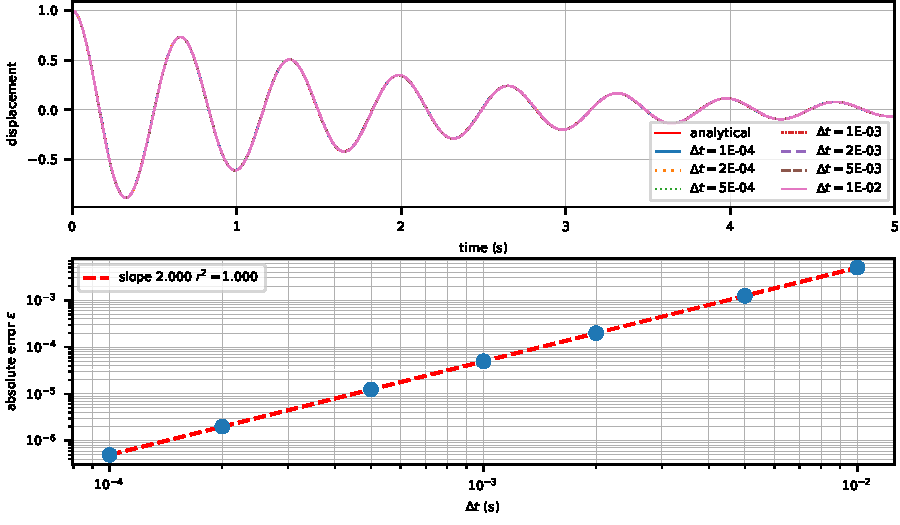
\includegraphics{PIC/UDD.SDOF.pdf}
    \caption{displacement history and error analysis of SDOF oscillator (free vibration)}\label{fig:sdof}
\end{figure}
\figref{fig:sdof_error} further shows the absolute error history of the SDOF system.
\begin{figure}
    \centering
    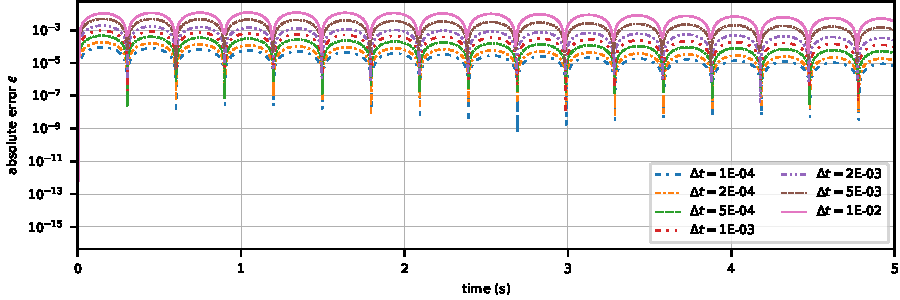
\includegraphics{PIC/UDD.SDOF.ERROR.pdf}
    \caption{absolute error history of SDOF oscillator (free vibration)}\label{fig:sdof_error}
\end{figure}